\chapter{Hauptteil}
\section{Figures und Floats}
\begin{wrapfigure}{L}{0.46\textwidth}
  \centering
	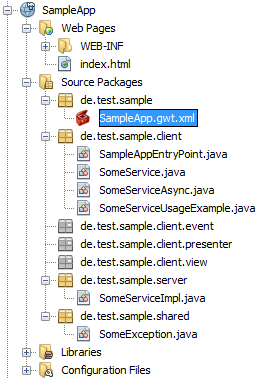
\includegraphics[]{figures/SampleAppProjektbaum}
    \caption{Projektbaum eines GWT Moduls}    
  \label{fig:projektbaum}
\end{wrapfigure}

\blindtext[2]

\begin{figure}[ht]
  \centering
	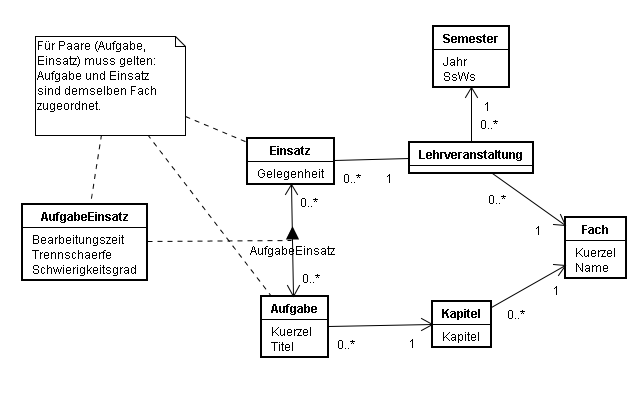
\includegraphics[width=\textwidth]{figures/DomainModel}
    \caption[Domänenmodell der Aufgabenpoolverwaltung]{Domänenmodell der Aufgabenpoolverwaltung.\\ \textbf{Quelle:} Prof. Dr. Robert Garmann}
  \label{fig:domainmodel}
\end{figure}

\begin{wrapfigure}{r}{0.45\textwidth}
  \vspace{-25pt}
  \centering
  \subfloat[Klassiches MVP]{\label{fig:mvp1}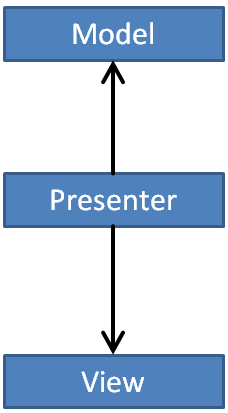
\includegraphics[scale=0.5]{figures/mvp1}}
  \quad
  \subfloat[MVP in der GWT-Architektur]{\label{fig:mvp2}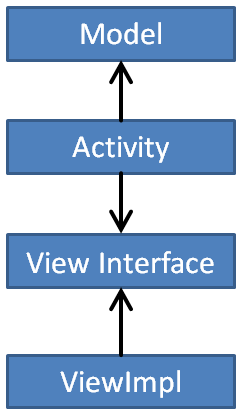
\includegraphics[scale=0.5]{figures/mvp2}}
    \caption{MVP nach \cite{GuUn2010}}
  \label{fig:mvp}  
  \vspace{-15pt}
\end{wrapfigure}

\blindtext[2]

\section{Listings}

Code wird für Java hervorgehoben. Ebenso inline-code wie dieser: \lstinline|public void essen() { System.out.println("esse"); }|

\lstinputlisting[float,label=lst:requestfactory,caption={Verwendung der RequestFactory beim Client\cite{GWT_REQ}}]{code/requestfactory.java}


\lstinputlisting[label=lst:uibinder_xml,language=xml,caption={Die XML-Beschreibung eines einfachen Widgets}]{code/HelloWidgetWorld.ui.xml}

Die Angabe von \lstinline|float| in den Attributen von \lstinline|\lstinputlisting| sorgt dafür, dass Quelltext nicht umgebrochen wird. 


\section{Sonstiges}
\subsection{Listen}
\begin{itemize}
\item eins
\item zwei
\item drei
\end{itemize}

\begin{enumerate}
\item eins
\item zwei
\item drei
\end{enumerate}

\subsection{Definitionen}
\begin{description}
\item[eins] ne zahl
\item[zwei] noch ne zahl
\item[drei] und noch eine
\end{description}

\subsection{Kompakte listen}
\section{Typographische Konventionen}
Die normalen Auflistungen haben viel whitespace oben und unten und zwischen drin. Mit \texttt{compactitem} kann dieser platz....
\begin{compactitem}
\item eins
\item zwei
\item drei
\end{compactitem}
.... verringert werden

\section{Tabellen}
\blindtext
\begin{table}[h]
	\centering
	\begin{tabular}{|l|l|l|}
\hline 
		Metrik 		  &Beschreibung 								&  Brauchbarkeit\\ 
\hline  
		\textbf{WMC}  &Gewichtete Methoden pro Klasse 				&  mäßig 		\\ 
\hline  
		\textbf{DIT}  &Tiefe im Vererbungsbaum 						&  hoch 		\\ 
\hline  
		\textbf{RFC}  &Antwortmenge einer Klasse 					&  hoch 		\\ 
\hline 
		\textbf{NOC}  &Zahl von Unterklassen 						&  hoch 		\\ 
\hline  
		\textbf{LCOM} &Mangel an Zusammenhang zwischen Methoden 	&  niedrig  	\\ 
\hline  
		\textbf{CBO}  &Kopplung zwischen Objektklassen 				&  hoch  		\\ 
\hline 
	\end{tabular} 
	\caption{Kennzahlen nach Chidamber \& Kemerer (aus \cite{Prech1999})}
	\label{tab:metrik}
\end{table}
